\documentclass[UTF8]{ctexart}
\usepackage{graphicx}
\usepackage{multirow}
\usepackage{booktabs}
\usepackage{indentfirst}
\setlength{\parindent}{2em}
\usepackage{color}
\definecolor{lbcolor}{rgb}{0.9,0.9,0.9}
\usepackage{listings}
\lstset{backgroundcolor=\color{lbcolor}}
\lstset{keywordstyle=\color[rgb]{0,0,1}}
\lstset{commentstyle=\color[rgb]{0.133,0.545,0.133}}
\lstset{stringstyle=\color[rgb]{0.627,0.126,0.941}}
\lstset{language=Matlab}
\lstset{numbers=left}
\lstset{breaklines=true}
\author{何舜成,厉丹阳}
\title{被动行走机器人混沌控制实验报告}
\begin{document}
\maketitle
\section{Lyapunov Exponent}
考虑初始值为$x(0)=x_{0}$的一条轨迹$x(t)=f(t,x_{0})$,以及初始值有小扰动的一条轨迹$x(t)+\delta x(t)=f(t,x_{0}+\delta x_{0})$,那么该演化轨迹对于初始值的敏感程度可以由以下公式衡量:\par
\begin{equation}
\parallel \delta x(t)\parallel \approx e^{\lambda t}\parallel \delta x_{0}\parallel
\end{equation}
\par
上式中$\lambda$表征了两个轨道之间的分离程度,被称作Leading Lyapunov Exponent(主导李雅普诺夫指数),从大时间尺度上看,LLE可以由下式衡量:\par
\begin{equation}
\lambda \approx \frac{1}{t}ln\frac{\parallel\delta x(t)\parallel}{\parallel\delta x(0)\parallel}
\end{equation}
\par
考虑一个离散非线性动力学系统:\par
\begin{equation}
x_{k+1}=f(x_{k}),x_{k}\in R^{n}
\end{equation}
\par
设$J_{k}$为$f(x)$在$x=x_{k}$处线性化得到的矩阵,再定义\par
\begin{equation}
T_{k}=J_{k}\cdots J_{2}J_{1}
\end{equation}
\par
那么第$i$个Lyapunov Exponent可表示为:\par
\begin{equation}
\lambda_{i}=\lim_{k \to \infty}\frac{1}{k}ln|\mu_{i}(T_{k})|
\end{equation}
\par
其中$\mu_{i}(T_{k})$表示矩阵$T_{k}$的第$i$个特征值。\par
据此原理则可以估计仿真程序中机器人行走的LLE。本程序中仿真了机器人走的1500步,取最后64步计算对应状态的Jacobian矩阵,累乘之后求特征值,取绝对值,取对数,除以矩阵数目64。可以得到4个Lyapunov Exponent(状态变量为4维),数值最大的即为LLE。仿真实验中观察斜坡角度$\gamma$对于被动行走机器人步态的影响,增大$\gamma$后机器人步态逐渐由单周期分叉为二周期,二周期分叉为四周期,四周期逐渐过渡为混沌步态。下图是$\gamma$变化对于机器人每步周期的影响。\par
\begin{figure}[htbp]
\centerline{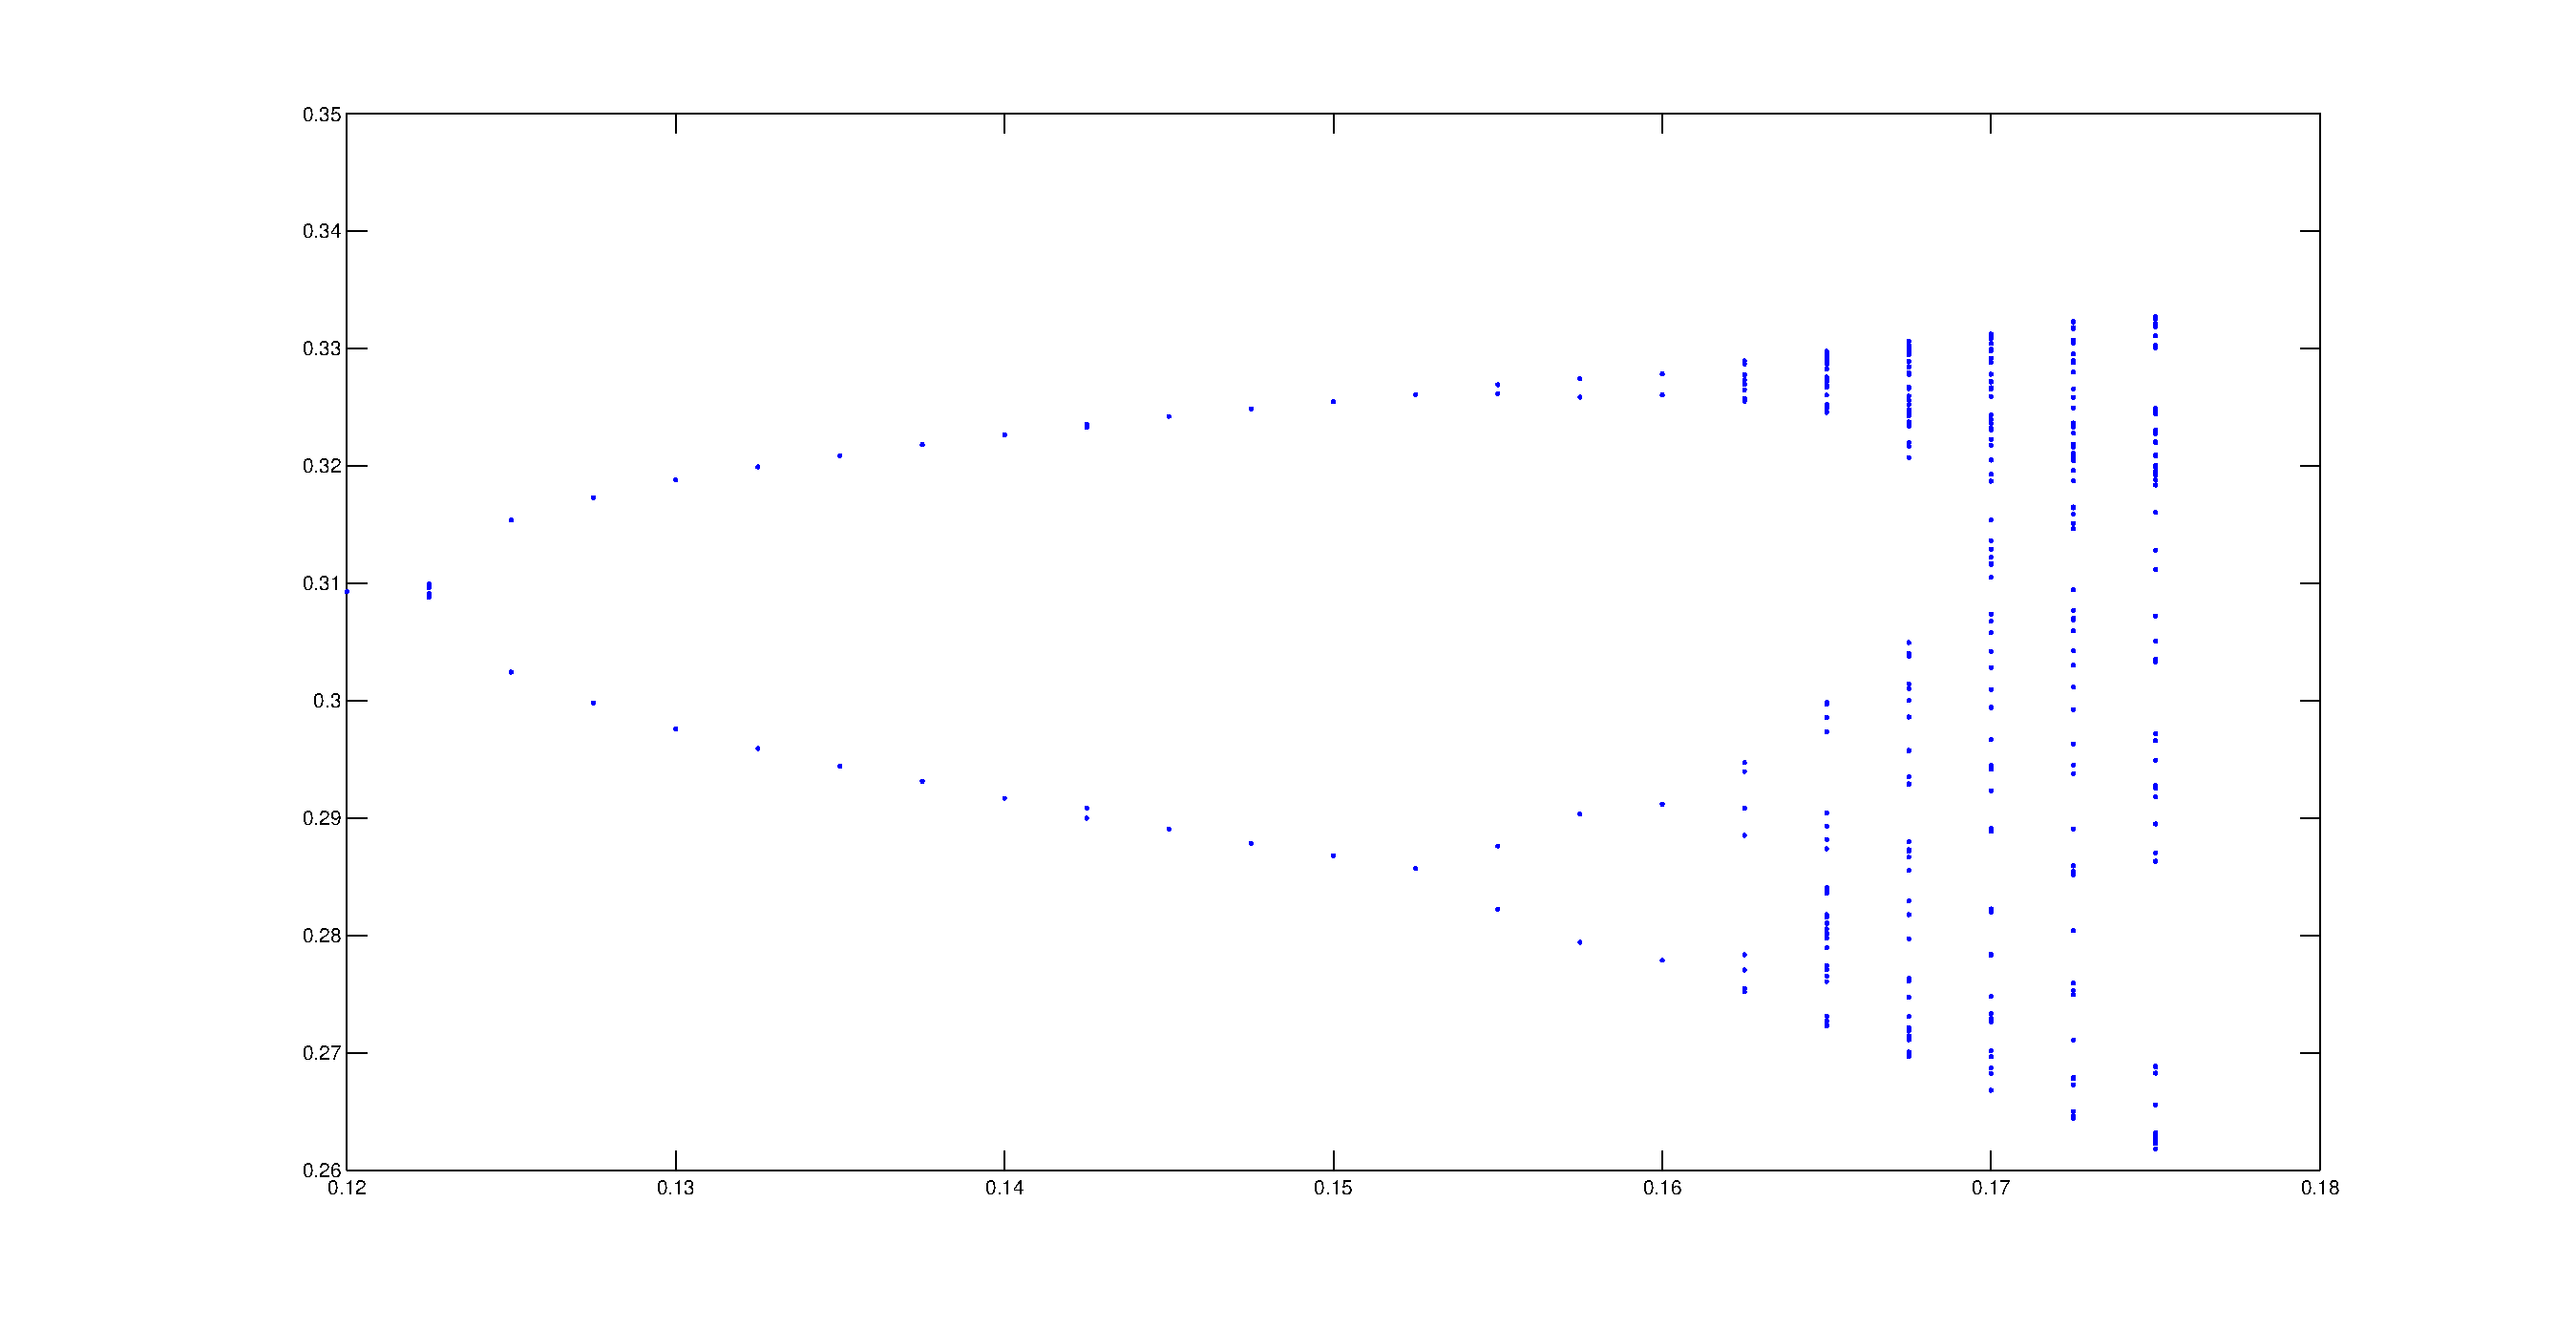
\includegraphics[width=\textwidth]{chaos.eps}}
\caption[]{$\gamma$变化导致的步态分叉与混沌现象}
\end{figure}
\par
大致可以看出,$\gamma=0.122$附近,步态由单周期变为二周期;$\gamma=0.153$附近,步态由二周期变为四周期;$\gamma=0.162$附近,步态变为多周期;$\gamma=0.165$附近基本变为混沌。图2是LLE随$\gamma$变化的曲线。\par
该曲线与之前的图较为一致,需要指出的是,在稳定状态下(单周期或多周期),LLE小于0,即所有Lyapunov Exponent都小于0;在混沌状态下,LLE大于0;LLE等于0的点会发生状态转换,产生分叉或进入混沌。\par
\begin{figure}[htbp]
\centerline{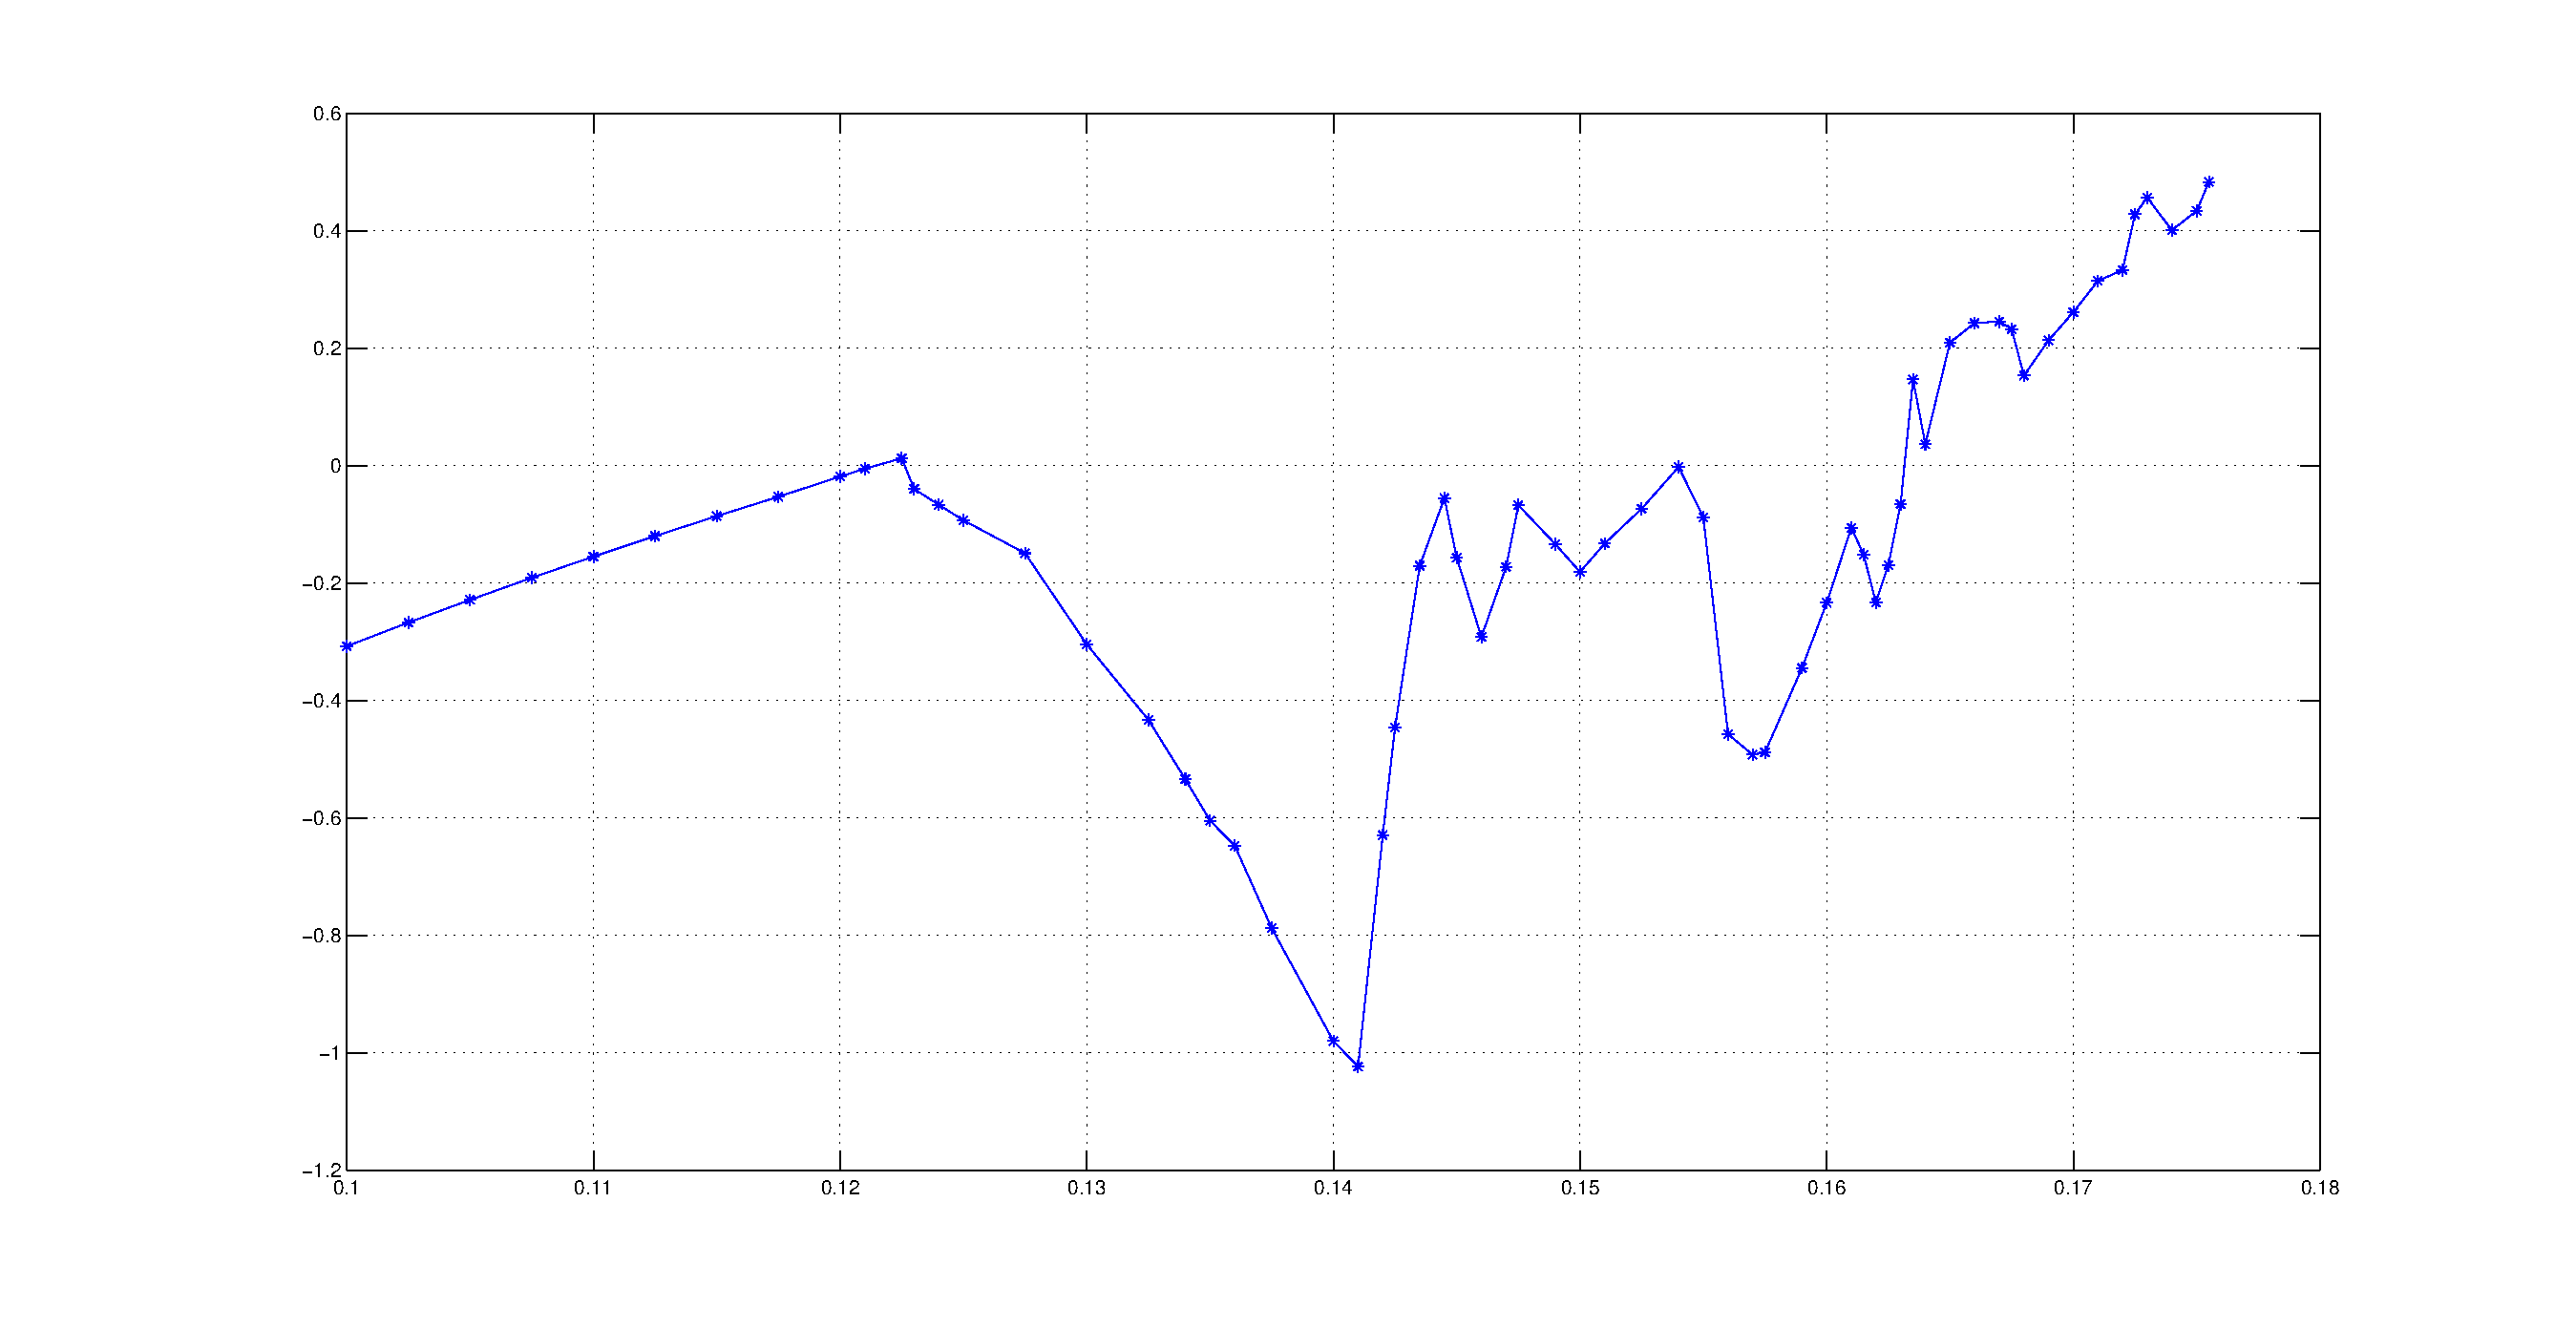
\includegraphics[width=\textwidth]{LyapunovExponent.eps}}
\caption[]{LLE随$\gamma$变化的曲线图}
\end{figure}
\par
\section{Chaos Control}
机器人在单周期步态下,状态演化在状态空间中的轨迹是闭合的环,被称为极限环。取机器人摆动腿触地的一瞬间为庞加莱截面,那么截面上的状态向量是离散非线性动力学系统方程(3)的不动点。在非单周期步态情况下,方程(3)的不动点仍然可以求出来,但该不动点是不稳定的。在不动点$s^{*}$处进行线性化,得到Jacobian矩阵$J^{*}=\partial f/\partial s^{*}$。易知,当$J^{*}$的特征值全部在单位圆内时,机器人表现为稳定的单周期步态,出现一定扰动时,状态轨线也会逐渐收敛与极限环;当$J^{*}$有特征值在单位圆外时,不动点不稳定,此时机器人可能表现出多周期步态(分叉)、混沌或倒下,状态轨线不会收敛到极限环上;当$J^{*}$有特征值在单位圆上时,Jacobian矩阵无法判断稳定性,需要更高阶的项来确定。\par
因此当机器人出现分叉或混沌步态时,跨步方程(stride function)不动点的Jacobian矩阵至少有一个特征值(或系统极点)落在单位圆外,选取一个控制量,可能可以通过状态反馈的方法将单位圆外的极点配置到单位圆内来,并可能通过极点配置改善动态品质。\par
本次仿真实验中,选取机器人质心在前后方向的位置(参数B)作为变化量,即观察参数B变化导致机器人步态的改变,直至出现分叉和混沌。然后将斜坡角度$\gamma$作为控制量,将分叉和混沌抑制到不动点(极限环)上去。\par
\subsection{Linearization}
原离散非线性方程为:\par
\begin{equation}
S_{n+1}=f(S_{n},\gamma)
\end{equation}
\par
在$\gamma^{*}$下,不动点$S^{*}$满足如下方程:\par
\begin{equation}
S^{*}=f(S^{*},\gamma^{*})
\end{equation}
\par
选定控制量之后可以列出如下线性化模型:\par
\begin{equation}
S^{*}=AS^{*}+B\gamma^{*}+F\omega
\end{equation}
\par
其中$\omega$是除控制量$\gamma$之外的扰动量。\par
在$S^{*}$和$\gamma^{*}$附近给一个小扰动$\Delta S$和$\Delta\gamma$,可以得到下式:\par
\begin{equation}
\Delta S_{n+1}=A\Delta S_{n}+B\Delta\gamma
\end{equation}
\par
\subsection{Feedback}
在不动点附近若出现了微小扰动$\Delta S$,依据状态反馈,可令控制量满足下式:\par
\begin{equation}
\Delta\gamma = -k\Delta S
\end{equation}
\par
其中$k$为待求量,代入原方程得:\par
\begin{equation}
\Delta S_{n+1}=(A-Bk)\Delta S_{n}
\end{equation}
\par
选取合适的$k$使得$A-Bk$的极点落在单位圆内,从而使不动点周围的微小扰动随步数增加而衰减到0。在$\Sigma(A,B)$完全可控时,可以选择$k$使得$A-Bk$的极点位于任意位置。当$\Sigma(A,B)$不完全可控时,可控性矩阵$Q_{C}=[B,AB,A^{2}B,A^{3}B]$不满秩,$r=rank(Q_{C})$即为可控状态数,亦即可以配置极点的自由度为$r$。\par
\subsection{Simulation}
首先对机器人质心前后位置B进行扫描,观察分叉和混沌现象。而后得到图3。\par
\begin{figure}[htbp]
\centerline{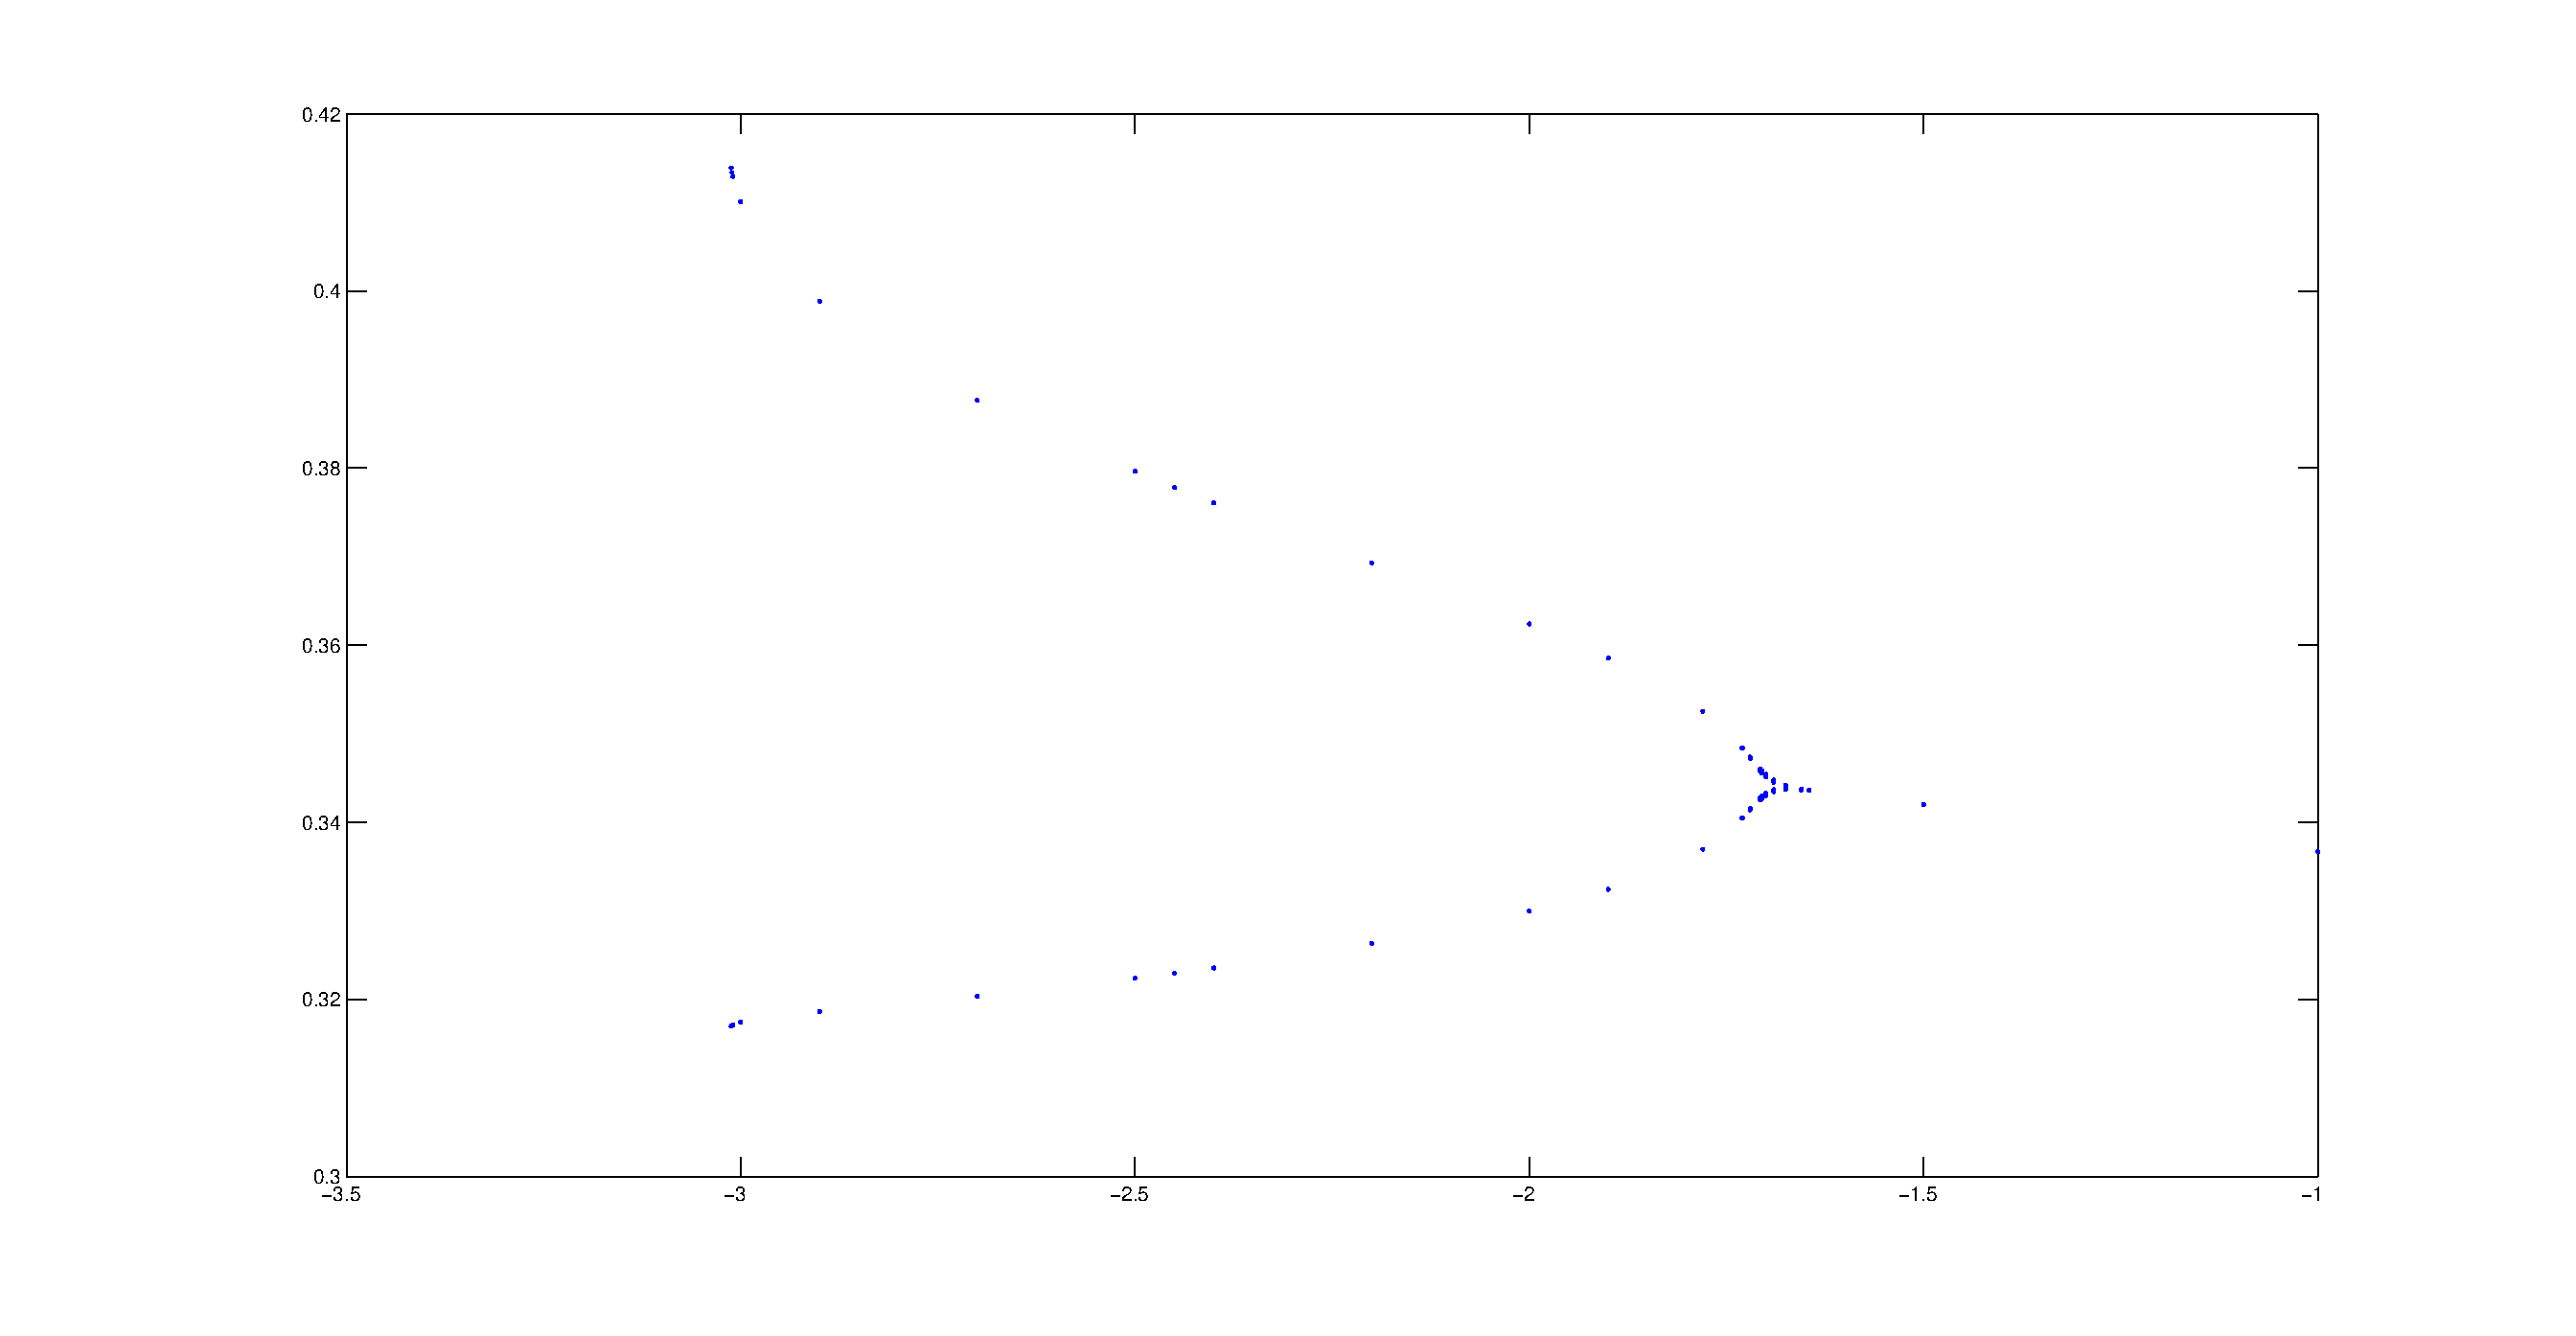
\includegraphics[width=\textwidth]{Bifurcation.eps}}
\caption[]{质心位置B引起的分叉现象}
\end{figure}
\par
可以看到随着B的减小,二分叉现象出现,然而在出现四分叉和混沌之前机器人倒掉,无法继续观察分叉和混沌。计算在不同参数B下的LLE如图4,只当$\Delta B\approx -1.7$时接近0,其余均小于0,辅助证明了机器人步态只出现了二分叉,而没有多分叉和混沌。然而接下来可以考虑状态反馈配置极点抑制二分叉。\par
\begin{figure}[htbp]
\centerline{\includegraphics[width=\textwidth]{Lyapunov.jpg}}
\caption[]{LLE随质心位置B变化的曲线}
\end{figure}
依据式(9),令$\Delta\gamma=0$,依次给状态变量$S_{n}$的各个分量加扰动$\Delta s_{i}=10^{-4}$,测得$\Delta S_{n+1}$,即可近似计算出$S_{n}$对应的Jacobian矩阵A。令$\Delta S=0$,给$\gamma$施加扰动$\Delta\gamma=10^{-4}$,测得$\Delta S_{n+1}$,可近似计算出矩阵B。\par
根据分叉状态下的Jacobian矩阵A的极点,选取期望极点[-0.8 0.5 -0.05 0],计算得到反馈矩阵$k$,再对参数B进行扫描,得到图5的抑制结果。\par
\begin{figure}[htbp]
\centerline{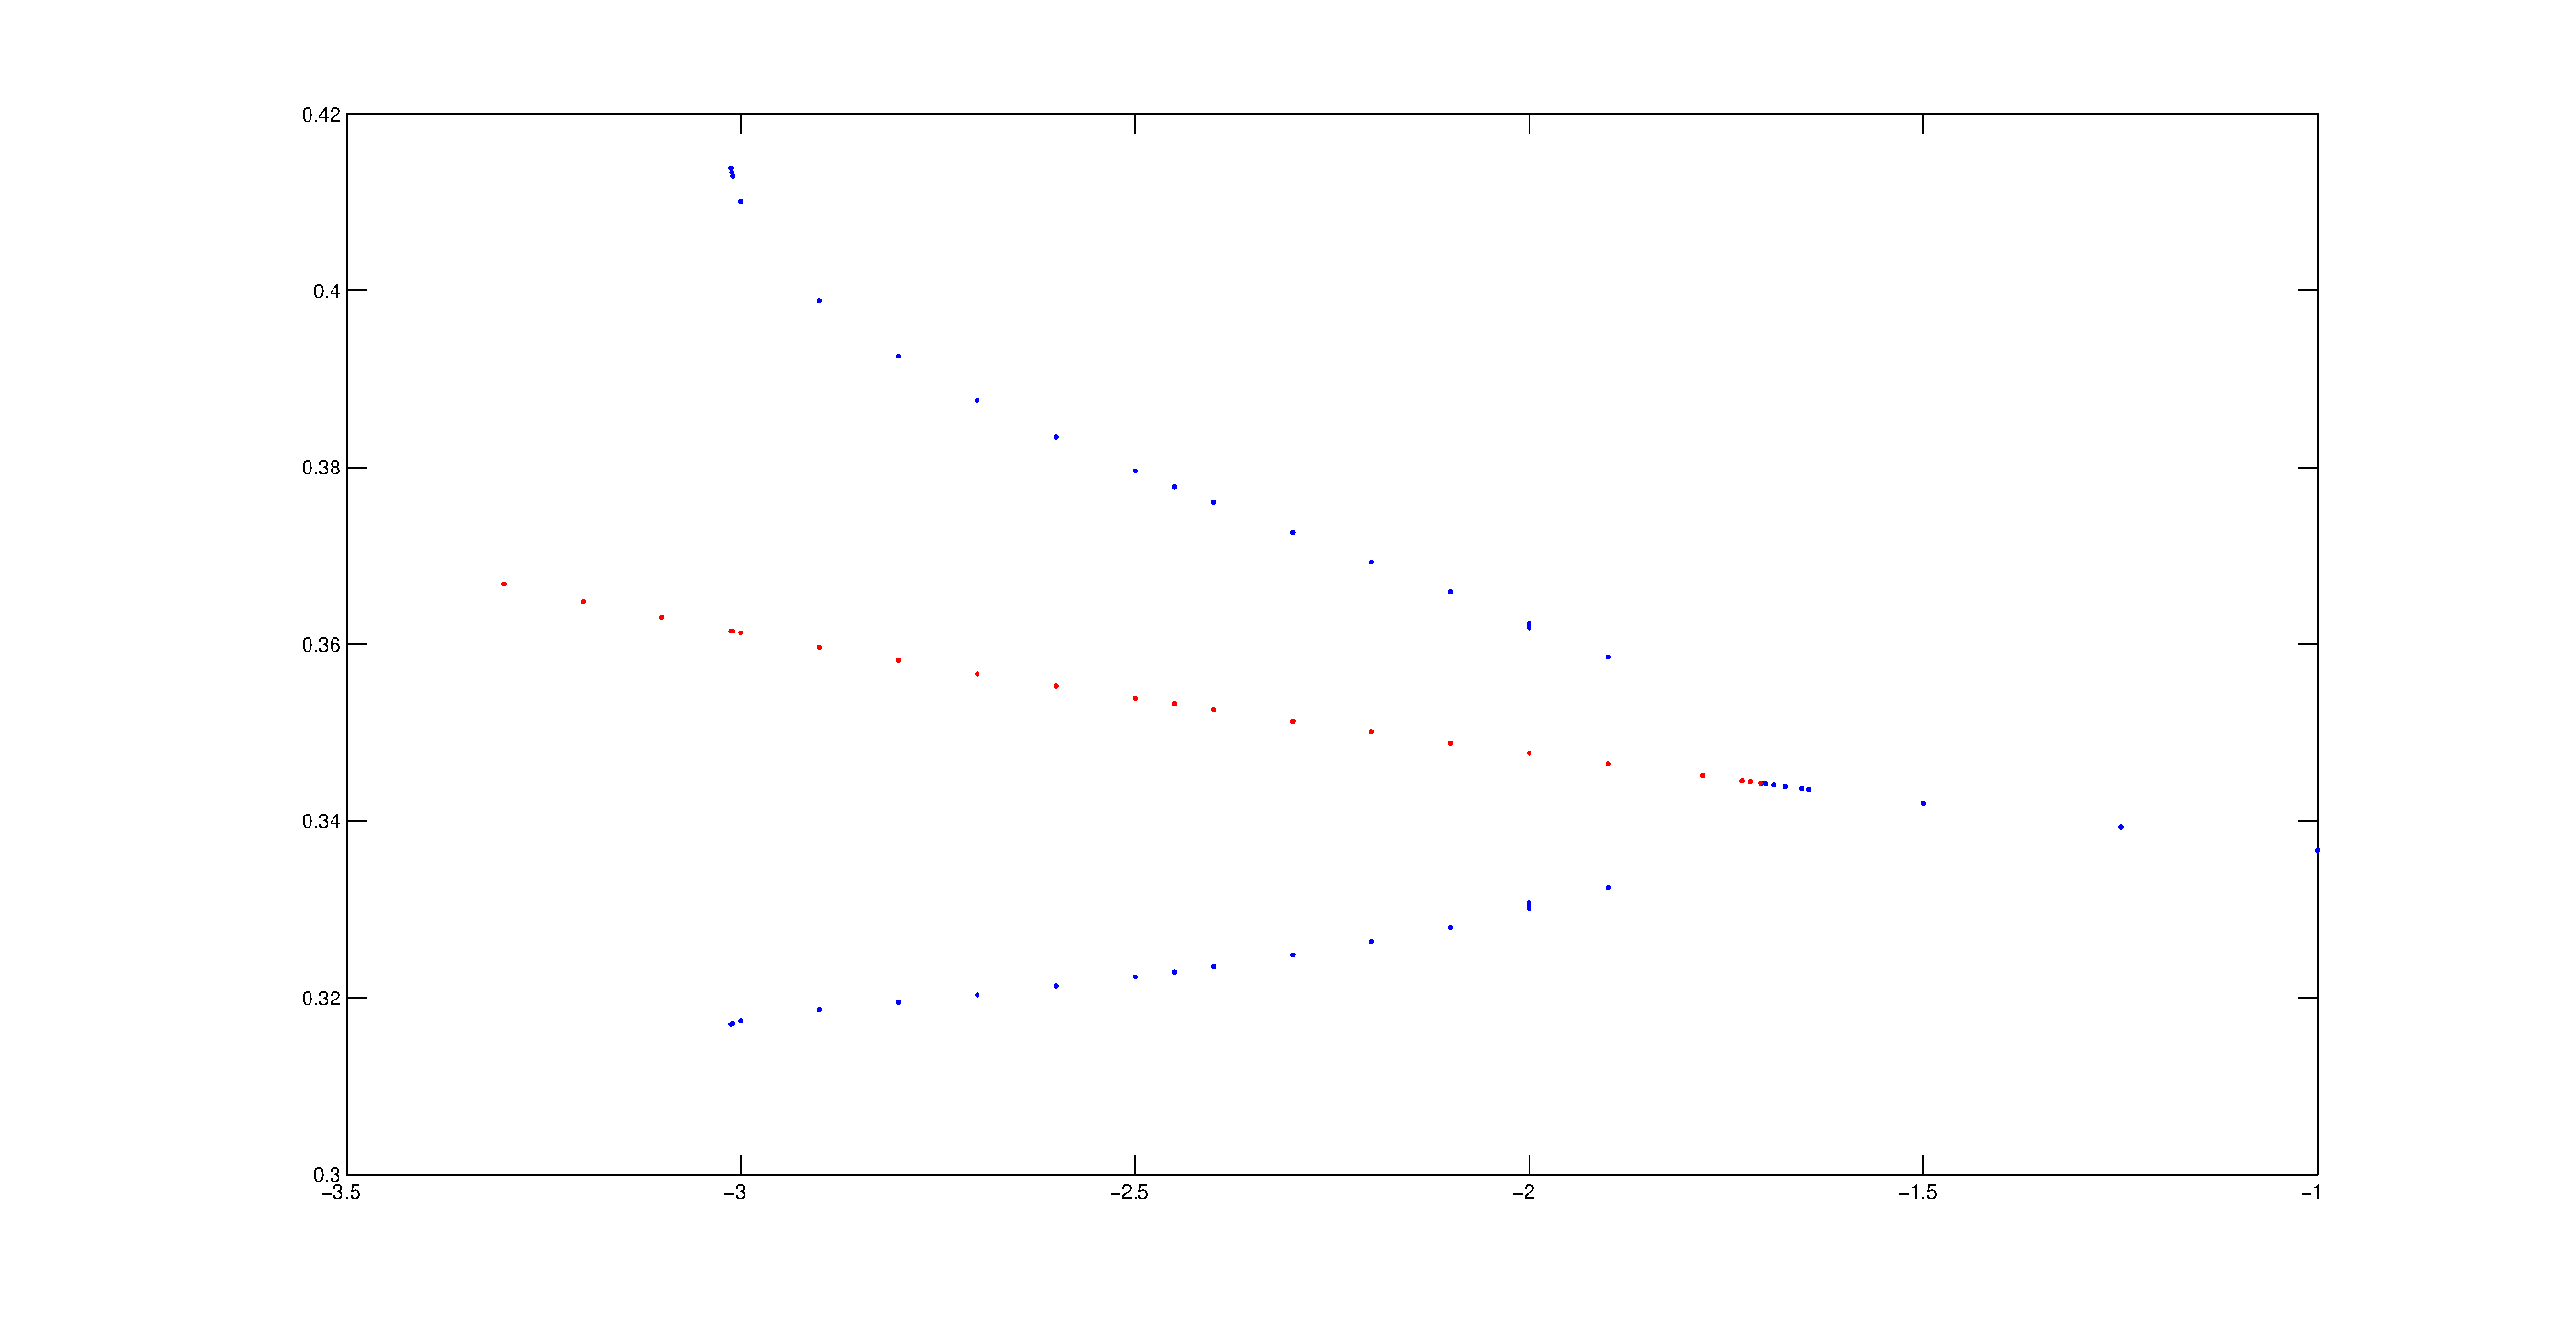
\includegraphics[width=\textwidth]{bifur&depr.eps}}
\caption[]{分叉抑制效果}
\end{figure}
\par
可以清楚的看到,在增加反馈之后,二分叉被抑制到原不动点上,并且在之前不能正常行走的$\Delta B$的取值上,机器人仍然可以在不动点上稳定行走。经过分析可以认为该控制方案是成功的。\par
\subsection{Discussion}
前述控制方案中期望极点被设置为[-0.8 0.5 -0.05 0],这是根据经验得到的一个方案。在某个会出现二分叉的点上计算Jacobian矩阵特征值为[-1.1864 0.6943 -0.0514 0],而可控性矩阵$Q_{C}$的秩为3,极点不能任意配置,因此可以尝试不动极点0,将两个较大的极点配小,尝试可知该极点配置方案可以计算出反馈矩阵$k$,且可以成功抑制分叉,因此是较为合适的。\par
另外需要关注的方面是控制的动态性能,在不加控制的情况下,机器人在稳定行走一段时间后逐渐发散,最后形成稳定的二周期步态(图6)。\par
\begin{figure}[htbp]
\centerline{\includegraphics[width=\textwidth]{NCC.jpg}}
\caption[]{不加控制时的二分叉步态}
\end{figure}
\par
仿真中试验了四组参数,分别是:\par
参数一:[-0.8 0.7 -0.05 0]\par
参数二:[-0.9 0.7 -0.05 0]\par
参数三:[-0.8 0.5 -0.05 0]\par
参数四:[-0.8 0.7 0.05 0]\par
得到不同的控制图谱:\par
\begin{figure}[htbp]
\centerline{\includegraphics[width=\textwidth]{CC-par1.jpg}}
\caption[]{使用参数一时的控制图谱}
\end{figure}
\begin{figure}[htbp]
\centerline{\includegraphics[width=\textwidth]{CC-par2.jpg}}
\caption[]{使用参数二时的控制图谱}
\end{figure}
\begin{figure}[htbp]
\centerline{\includegraphics[width=\textwidth]{CC-par3.jpg}}
\caption[]{使用参数三时的控制图谱}
\end{figure}
\begin{figure}[htbp]
\centerline{\includegraphics[width=\textwidth]{CC-par4.jpg}}
\caption[]{使用参数四时的控制图谱}
\end{figure}
\par
参数一、二、四下控制均出现了误差,参数二下逐渐发散,可能将趋于不稳定,参数四下过渡时间较长,震荡较多。参数三下控制既没有出现误差,又不产生震荡,控制品质好于其他几组参数,因此选定该组参数作为抑制分叉的控制措施。极点配置对于控制品质的影响的机制尚不明确。\par

\end{document}